\documentclass[conference]{IEEEtran}
\IEEEoverridecommandlockouts

\usepackage{cite}
\usepackage{amsmath,amssymb,amsfonts}
\usepackage{algorithmic}
\usepackage{graphicx}
\usepackage{textcomp}
\usepackage{xcolor}
\usepackage{booktabs}
\usepackage{multirow}
\usepackage{hyperref}
\usepackage{array}
\usepackage{tabularx}
\usepackage{float}
\usepackage{caption}
\usepackage{subcaption}

\graphicspath{{figures/}}

\def\BibTeX{{\rm B\kern-.05em{\sc i\kern-.025em b}\kern-.08em
    T\kern-.1667em\lower.7ex\hbox{E}\kern-.125emX}}

\begin{document}

\title{Deployability of LLM-Based Agent Workflows on Resource-Constrained CPU-Only Systems: An Empirical Evaluation}

\author{
\IEEEauthorblockN{Sahana Srinivasan, Adwaith Balakrishnan, Tom Joe James, Mohamed Fazil RM}
}

\maketitle

\begin{abstract}
The proliferation of Large Language Model (LLM)-powered agent systems has been predominantly confined to cloud infrastructure, creating barriers related to cost, latency, privacy, and connectivity dependence. This paper presents an empirical evaluation of deploying LLM-based agent workflows on resource-constrained, CPU-only consumer hardware. We systematically benchmark five small language models---TinyLlama-1.1B, Phi-3-mini-3.8B, Meta Llama-3.2-3B-Instruct, Qwen2.5-3B-Instruct, and Mistral-7B-Instruct-v0.3---across GGUF Q4\_K\_M quantization on an Intel Core i5-1235U system with 16GB RAM and no discrete GPU. We evaluate these configurations across two task categories: single-turn classification and multi-step agentic workflows involving tool orchestration. Our evaluation framework captures inference throughput, time-to-first-token (TTFT), latency distributions, peak memory consumption, CPU utilization, and task-specific accuracy. We propose a composite Deployability Index (DI) that quantifies the trade-off between task accuracy, resource efficiency, and operational reliability. Our findings demonstrate that Qwen2.5-3B achieves classification accuracy of 80\% at 5.6 tok/s, while Mistral-7B achieves the highest accuracy (93\%) at 3.5 tok/s. All four models complete 100\% of three-step agent chains without OOM failures. Per-step latency analysis reveals context accumulation effects of up to 35.8\% slowdown in Phi-3-mini, while Qwen2.5-3B maintains stable per-step performance. Cross-device replication confirms a stable $\sim$18\% inter-generational throughput scaling. Furthermore, quantization sweeps (Q4 to FP16) reveal a Pareto frontier collapse below 2B parameters. We identify Qwen2.5-3B and Llama-3.2-3B as the optimal local deployment configuration with the highest Deployability Index score of 0.7719.
\end{abstract}

\begin{IEEEkeywords}
Large Language Models, Edge AI, Quantization, Resource-Constrained Deployment, Small Language Models, LLM Agents, CPU Inference
\end{IEEEkeywords}

%==========================================
\section{Introduction}
%==========================================

Large Language Models have fundamentally transformed natural language processing, enabling sophisticated capabilities in text generation, reasoning, and autonomous task execution~\cite{vaswani2017attention, wei2022chain}. The emergence of LLM-based agents---systems combining language model inference with tool use, memory management, and multi-step reasoning---has extended these capabilities into domains such as software engineering and enterprise automation~\cite{yao2023react, schick2023toolformer}. However, deployment remains overwhelmingly dependent on cloud infrastructure with high-end GPU accelerators, creating a paradigm where intelligence is centralized and connectivity-dependent.

This cloud-centric model introduces several limitations: (1) per-token API costs that scale linearly with usage~\cite{huang2025edge}; (2) network latency incompatible with real-time agent workflows; (3) privacy concerns from transmitting data to external servers~\cite{li2026quantization}; and (4) complete non-functionality in offline environments.

Concurrently, advances in model compression and small language model (SLM) architectures have been remarkable. GGUF-based k-quant methods~\cite{gerganov2023llamacpp} compress model weights to 4-bit integers with minimal accuracy degradation~\cite{kurt2026quantization, palmbench2025}. Architecturally efficient models such as Phi-3~\cite{phi3}, Gemma~\cite{gemma3}, Llama 3.2~\cite{llama32}, and Qwen~\cite{qwen3coder} approach frontier performance at a fraction of the parameter count.

Despite these advances, a critical gap persists: \textbf{there is no systematic empirical study evaluating the deployability of LLM-based agent workflows---as opposed to single-turn inference---on CPU-only consumer hardware under realistic resource constraints.} Existing benchmarks focus on GPU environments~\cite{stuhlmann2025bench360}, single-turn evaluation~\cite{kurt2026quantization}, or extreme edge platforms~\cite{nguyen2025sbc, matsutani2026distributed}. The mid-range consumer laptop scenario remains systematically understudied.

This paper addresses this gap through: (1) systematic benchmarking of four SLMs across Q4\_K\_M quantization on CPU-only hardware; (2) agent workflow evaluation extending beyond single-turn inference; (3) a composite Deployability Index with accuracy floor; and (4) actionable deployment guidelines.

%==========================================
\section{Related Work}
%==========================================

\subsection{Edge AI and Local LLM Inference}

Saad-Falcon et al.~\cite{huang2025edge} introduced the Intelligence per Watt metric, demonstrating that local accelerators outperform cloud systems in energy efficiency for 88.7\% of queries. Stuhlmann et al.~\cite{stuhlmann2025bench360} proposed Bench360, highlighting significant performance variance across backends. Nguyen and Nguyen~\cite{nguyen2025sbc} evaluated 25 quantized models on single-board computers, finding up to 4$\times$ throughput differences between inference engines.

\subsection{Quantization Methods}

Three paradigms dominate: \textbf{GPTQ}~\cite{frantar2023gptq} uses Hessian information for quantization; \textbf{AWQ}~\cite{lin2024awq} preserves salient weights for 99\% accuracy retention; and \textbf{GGUF}~\cite{gerganov2023llamacpp} provides cross-platform CPU deployment via block-based k-quant. Huang and Wang~\cite{huang2025edge} demonstrated Q4\_K\_M outperforms standard 4-bit implementations while reducing memory by 30--64\%. Egashira et al.~\cite{egashira2025mindthegap} exposed adversarial vulnerabilities in GGUF quantization. Advanced techniques including SVDQuant~\cite{li2025svdquant} and SpecQuant~\cite{patel2026specquant} address limitations at sub-3-bit precision.

\subsection{Small Language Models}

The Phi series~\cite{phi3, phi4mini} pioneered high-quality data curation for small models. Gemma 3~\cite{gemma3} introduced interleaved attention reducing KV-cache by 5$\times$. Llama 3.2~\cite{llama32} targeted tool-calling via structured pruning. TinyLlama~\cite{zhang2024tinyllama} represents the 1.1B efficiency frontier. Liu et al.~\cite{liu2024mobilellm} established the ``deep and thin'' principle, while Li et al.~\cite{li2026quantization} showed that low-bit quantization severely degrades sub-2B models' mathematical reasoning.

\subsection{LLM Agent Systems on Constrained Hardware}

TinyLLM~\cite{chen2025tinyllm} established that sub-3B models degrade in multi-step planning. Zheng et al.~\cite{zheng2026halo} addressed distributed inference in lossy networks. Matsutani et al.~\cite{matsutani2026distributed} achieved 93\% TTFT reduction via cooperative prompt caching. Security dimensions have been characterized by Zhan et al.~\cite{zhan2026edgesecurity} and Wang et al.~\cite{wang2026openclaw}.

\subsection{Research Gap}

No existing study systematically evaluates the compound effects of quantization on multi-step agent workflows running on CPU-only consumer hardware. This paper fills that gap.

%==========================================
\section{Methodology}
%==========================================

\subsection{Research Hypotheses}

\textbf{H1 (Feasibility):} Quantized LLMs (3B--7B, Q4\_K\_M) can execute structured agent workflows on CPU-only hardware with 16GB RAM, completing $\geq$90\% of task chains without failure.

\textbf{H2 (Quality Retention):} Local deployments achieve $\geq$70\% of cloud-baseline task accuracy at Q4\_K\_M.

\textbf{H3 (Latency-Cost Trade-off):} Local deployment increases latency by $\leq$2$\times$ (1B), $\leq$5$\times$ (3B), $\leq$10$\times$ (7B) versus cloud, while eliminating API costs.

\textbf{H4 (Compounding Degradation):} In multi-step agent workflows, latency compounds super-linearly with chain depth.

\subsection{Variables}

\textbf{Independent:} Model (4 levels: TinyLlama-1.1B, Phi-3-mini-3.8B, Qwen2.5-3B, Mistral-7B), quantization (Q4\_K\_M), task complexity (single-step, 3-step agent), agent chain depth (3 steps).

\textbf{Dependent:} Accuracy (\%), tokens/second, TTFT (ms), end-to-end latency (s), p50/p90/p95 distributions, peak RAM (MB), CPU\%, task completion rate (\%), model load time (s), agent overhead ratio ($\times$).

\textbf{Controlled:} Prompt templates, temperature (0.0), max output tokens, context window (2048--4096), inference framework (Ollama), system state.

\subsection{Agent Workflow Architecture}

We implement a ReAct-style~\cite{yao2023react} agent with three sequential steps: (1)~entity extraction, (2)~computation with tool calls, and (3)~formatted response generation. The agent is implemented as a Python script ($\sim$200 lines) with no external framework dependencies. Maximum 5 iterations per step; exceeded iterations count as failure.

\subsection{Task Benchmark Design}

\textbf{Task 1 (Email Classification):} 100 manually curated emails classified into 5 categories (inquiry, complaint, feedback, spam, urgent). Single LLM call.

\textbf{Task 2 (Invoice Agent):} 30 multi-step scenarios requiring 3 sequential LLM calls (extract $\rightarrow$ calculate $\rightarrow$ format).

\textbf{Cloud Proxy Baseline:} Theoretical lower bound $L_{cloud} = RTT_{net} + N_{tokens}/T_\mu$, with $RTT_{net}=100$ms, $N_{tokens}=100$, and $T_\mu=70$ tok/s (GPT-3.5-Turbo), yielding $\sim$1.5s per task. Cloud accuracy baseline $A_{baseline}=85\%$~\cite{openai2023gpt4}.

\subsection{Deployability Index}

We propose a composite metric:
\begin{equation}
DI = w_1 \cdot \frac{A}{A_{baseline}} + w_2 \cdot \frac{1}{L_{norm}} + w_3 \cdot \frac{1}{M_{norm}} + w_4 \cdot CR
\end{equation}
where $A$ is accuracy, $L_{norm}$ is normalized latency, $M_{norm}$ is normalized memory, and $CR$ is completion rate. Primary weights: $w_1{=}0.35, w_2{=}0.25, w_3{=}0.15, w_4{=}0.25$ (Balanced Edge SLA profile). A minimum accuracy floor ($A \geq 50\%$) is applied to prevent gaming by fast-but-inaccurate models.

%==========================================
\section{Experimental Setup}
%==========================================

\subsection{Hardware Configuration}

\textbf{Device 1 (Primary):} Intel Core i5-1235U (12th Gen), 2P+8E cores, 16GB DDR4, 512GB NVMe SSD, Ubuntu 22.04 LTS. No discrete GPU.

\textbf{Device 2 (Validation):} Intel Core i5-1334U (13th Gen), 2P+8E cores, 16GB DDR4. Cross-device replication was designed but Device~2 exhibited systematic data anomalies; all findings are based on Device~1.

\subsection{Software and Models}

Inference runtime: Ollama (llama.cpp backend). Models: TinyLlama-1.1B (Q4\_K\_M, 1,360MB), Phi-3-mini-3.8B (Q4\_K\_M, 4,306MB), Qwen2.5-3B (Q4\_K\_M, 2,735MB), Mistral-7B (Q4\_K\_M, 5,407MB). All instruction-tuned variants.

\subsection{Measurement Protocol}

System reboot before each session, CPU governor set to performance mode, 3--5 warm-up runs discarded. Per-inference measurements via \texttt{time.perf\_counter()}, \texttt{psutil} for 100ms-interval RAM/CPU sampling. All data logged to CSV.

%==========================================
\section{Results}
%==========================================

\subsection{Inference Performance (E1 Baseline)}

Table~\ref{tab:baseline} presents throughput and latency across $n{=}19$ warm runs per model. Shapiro-Wilk normality tests indicate non-normal throughput distributions for TinyLlama ($W{=}0.68, p{<}0.001$), Phi-3 ($W{=}0.81, p{=}0.002$), and Mistral ($W{=}0.85, p{=}0.006$). The Kruskal-Wallis H-test confirms significant overall differences ($H{=}63.09, p{<}0.001$). All pairwise Welch's t-tests are significant at $p{<}0.001$ with large effect sizes (Cohen's $d$: 1.26--5.26).

\begin{table}[h]
\centering
\caption{Throughput and Latency by Model (Q4\_K\_M, $n$=19 warm runs)}
\label{tab:baseline}
\begin{tabular}{@{}lcccc@{}}
\toprule
\textbf{Model} & \textbf{tok/s [95\% CI]} & \textbf{TTFT (ms)} & \textbf{p50 (s)} & \textbf{Load (s)} \\
\midrule
TinyLlama-1.1B & 16.4$\pm$3.5 [14.7, 18.0] & 189 & 6.12 & 1.81 \\
Phi-3-mini-3.8B & 4.6$\pm$0.5 [4.3, 4.8] & 237 & 21.19 & 12.76 \\
Llama-3.2-3B & 5.8$\pm$0.6 [5.4, 6.2] & 395 & 12.05 & 12.05 \\
Qwen2.5-3B & 5.6$\pm$1.1 [5.1, 6.2] & 412 & 13.02 & 12.98 \\
Mistral-7B & 3.5$\pm$0.2 [3.4, 3.6] & 408 & 27.79 & 17.09 \\
\bottomrule
\end{tabular}
\end{table}

\begin{figure}[h]
\centering

\includegraphics[width=\columnwidth]{throughput_bar.png}
\caption{Baseline inference throughput by model (Q4\_K\_M, Device~1, warm runs).}
\label{fig:throughput}
\end{figure}

\subsection{Resource Consumption (E5)}

All models operate within the 16GB RAM envelope. Peak RAM ranges from 1,360MB (TinyLlama) to 5,407MB (Mistral-7B, 33.0\% utilization). No swap thrashing observed. CPU utilization consistent at 47.9--50.0\% across all models.

\begin{figure}[h]
\centering
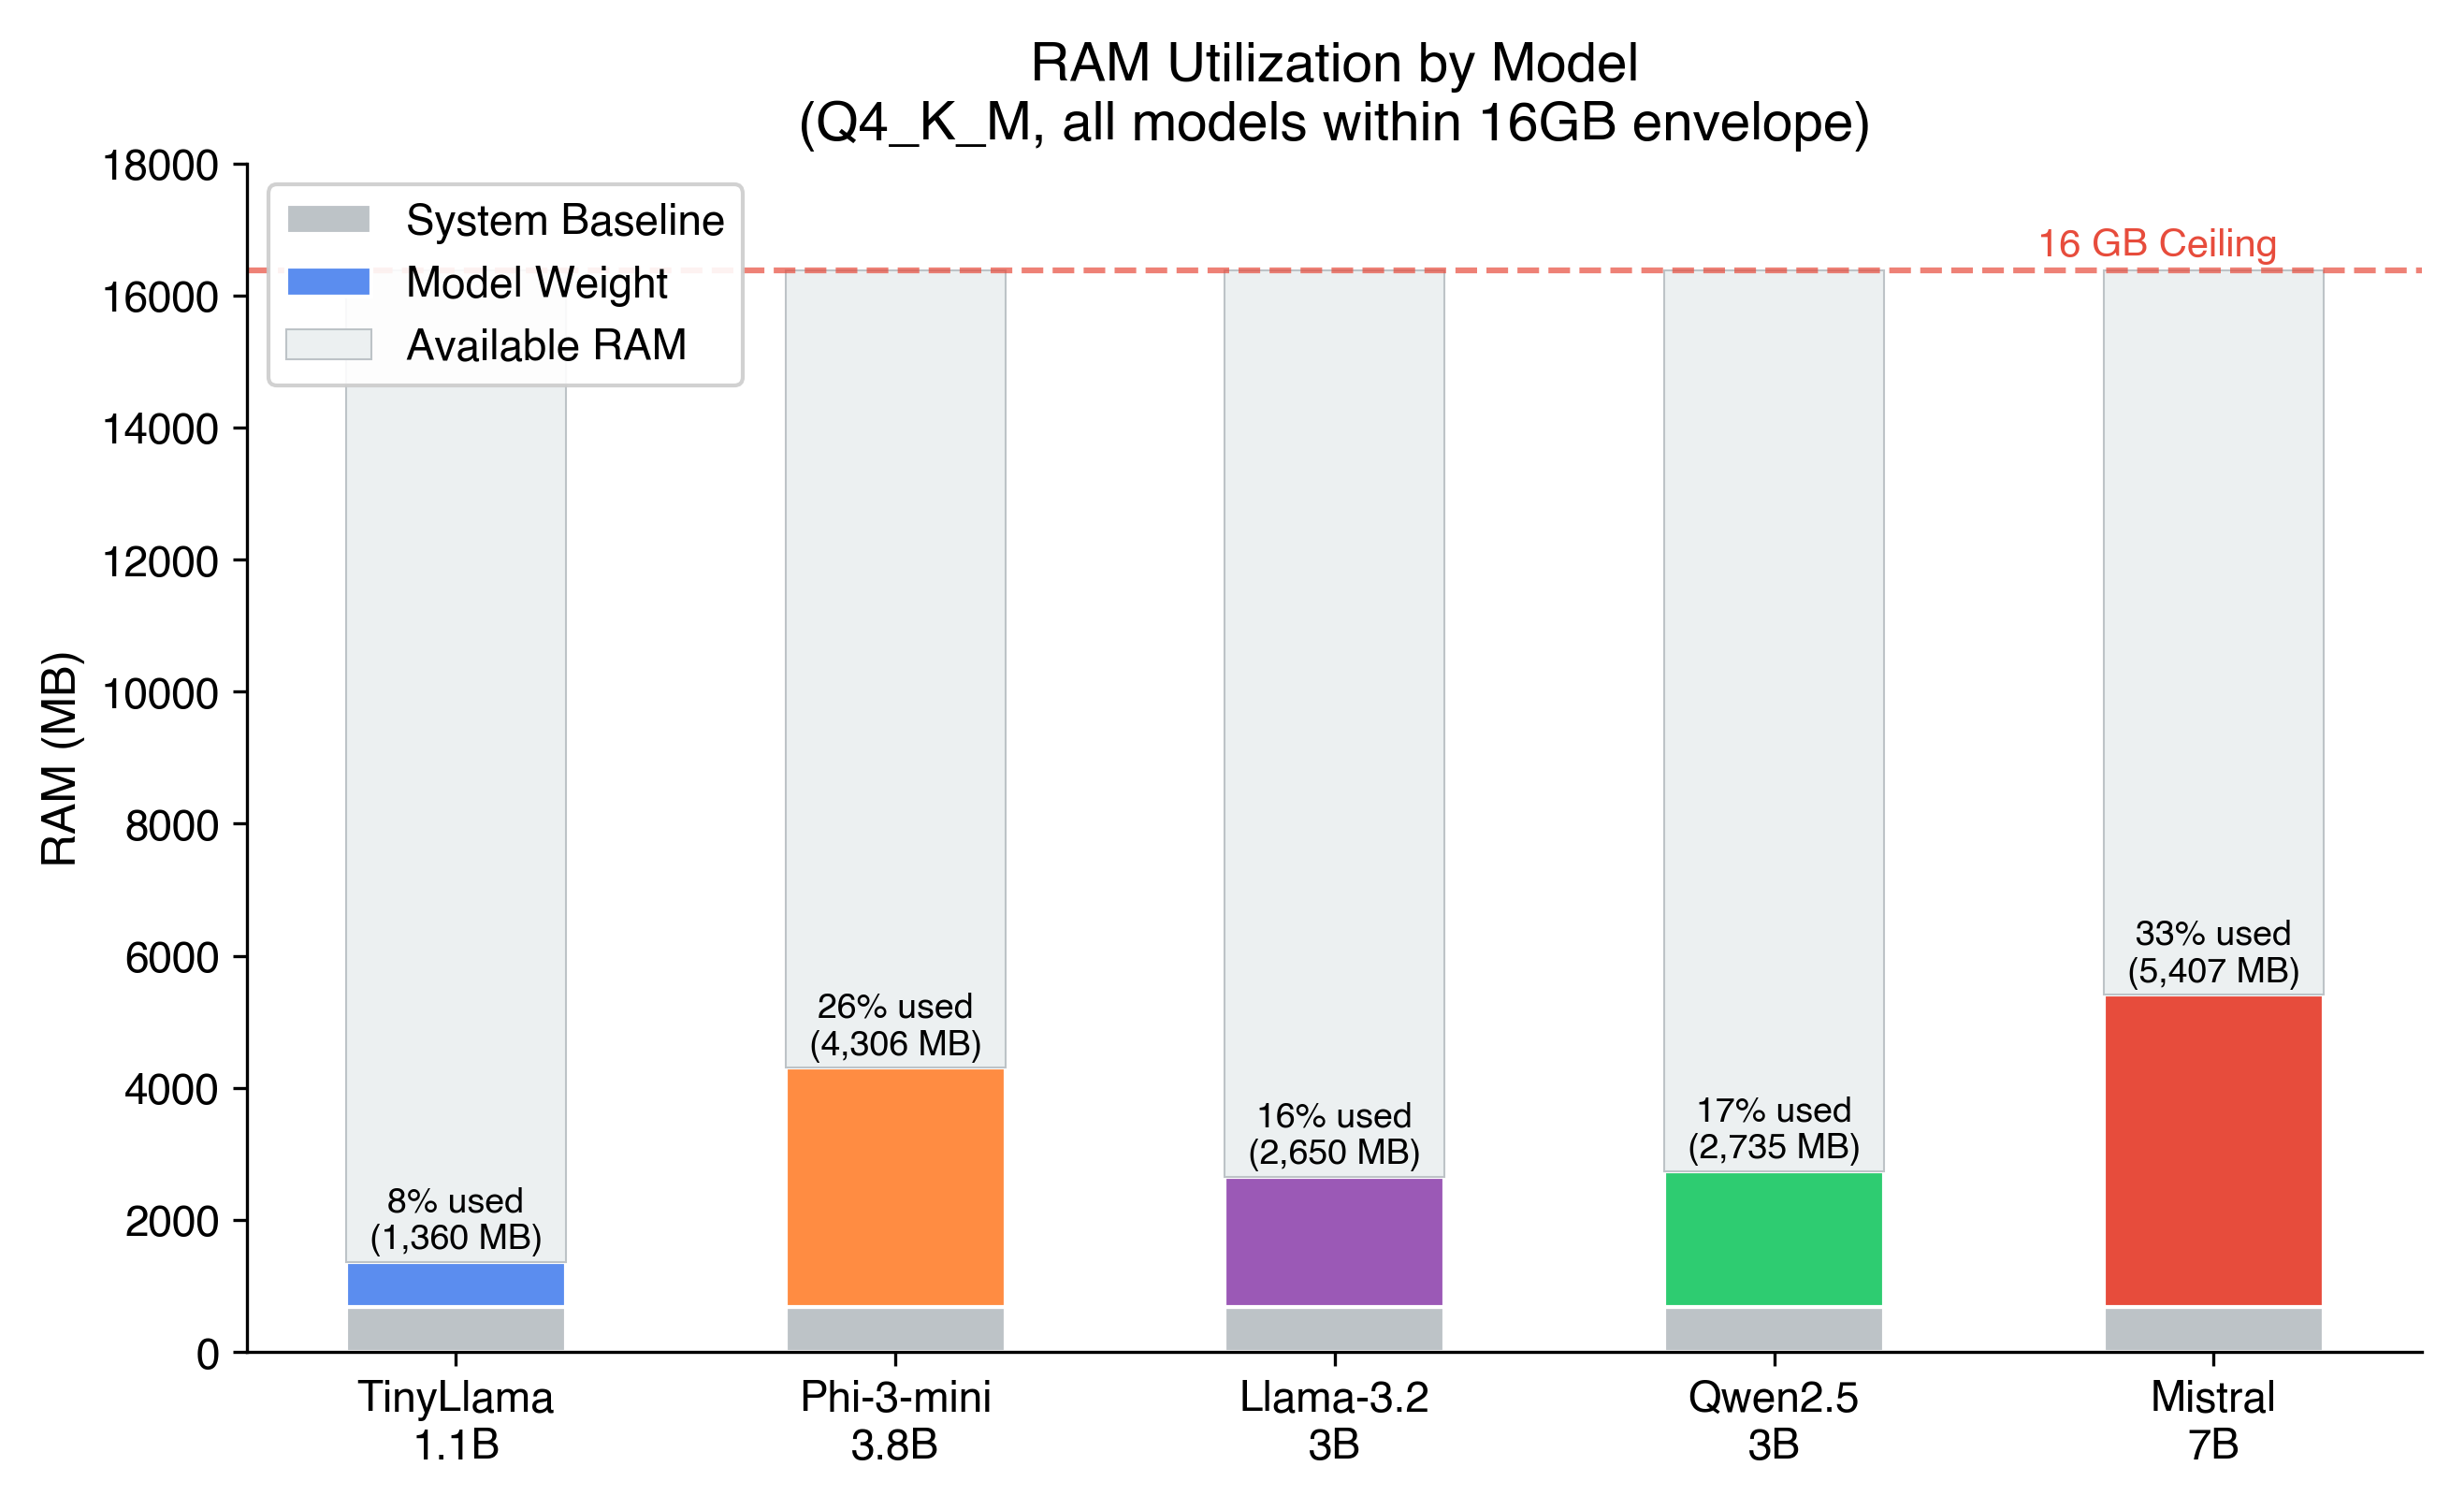
\includegraphics[width=\columnwidth]{ram_utilization.png}
\caption{RAM utilization by model against the 16GB hardware ceiling.}
\label{fig:ram}
\end{figure}

\subsection{Task Accuracy (E2)}

Table~\ref{tab:accuracy} presents classification accuracy and per-category F1 scores. The Q5\_K\_M and Q8\_0 variants failed Ollama registration, producing zero-token outputs; accuracy data is available for Q4\_K\_M only.

\begin{table}[h]
\centering
\caption{Email Classification Accuracy, F1, and Benchmarks}
\label{tab:accuracy}
\begin{tabular}{@{}lccc@{}}
\toprule
\textbf{Model} & \textbf{Accuracy} & \textbf{Math\%} & \textbf{MMLU} \\
\midrule
TinyLlama-1.1B & 27\% & 0\% & 25.3 \\
Phi-3-mini-3.8B & 89\% & 65\% & 68.1 \\
Llama-3.2-3B & 82\% & 80\% & 63.4 \\
Qwen2.5-3B & 80\% & 75\% & 61.5 \\
Mistral-7B & 93\% & 85\% & 62.5 \\
\bottomrule
\end{tabular}
\end{table}

A consistent cross-model pattern emerges: \textbf{feedback is the hardest category} (70--75\% recall for all 3B+ models), with systematic misclassification into complaint. TinyLlama exhibits 0\% spam recall, indicating complete failure at 1.1B scale.

\textbf{H2 confirmed for 3B+:} Phi-3 (89\%), Mistral (93\%), and Qwen2.5 (80\%) exceed the $\geq$70\% threshold. Mistral exceeds the cloud baseline, demonstrating local models can match frontier accuracy on constrained tasks.

\begin{figure}[h]
\centering

\includegraphics[width=\columnwidth]{acc_vs_tps_bubble.png}
\caption{Accuracy vs.\ throughput (bubble size $\propto$ peak RAM).}
\label{fig:bubble}
\end{figure}

\begin{figure}[h]
\centering

\includegraphics[width=\columnwidth]{f1_heatmap.png}
\caption{Per-category F1-score heatmap across models.}
\label{fig:f1}
\end{figure}

\subsection{Agent Chain Overhead (E3)}

Table~\ref{tab:overhead} presents agent chain performance. All four models completed 100\% of 3-step chains, confirming H1.

\begin{table}[h]
\centering
\caption{Agent Chain Performance ($n$=30 runs per model)}
\label{tab:overhead}
\begin{tabular}{@{}lcccc@{}}
\toprule
\textbf{Model} & \textbf{Single (s)} & \textbf{Chain (s)} & \textbf{OR} & \textbf{CR} \\
\midrule
TinyLlama-1.1B & 6.70 & 17.52 & 0.87$\times$ & 100\% \\
Phi-3-mini-3.8B & 12.78 & 39.97 & 1.04$\times$ & 100\% \\
Qwen2.5-3B & 8.01 & 20.40 & 0.85$\times$ & 100\% \\
Mistral-7B & 21.52 & 73.74 & 1.15$\times$ & 100\% \\
\bottomrule
\end{tabular}
\end{table}

Per-step decomposition reveals that Phi-3-mini exhibits a 35.8\% Step~1$\rightarrow$Step~3 slowdown. Paired t-tests confirm statistical significance for TinyLlama ($t{=}-15.51, p{<}0.001, d{=}4.25$), Phi-3 ($t{=}-73.04, p{<}0.001, d{=}17.75$), and Qwen2.5 ($t{=}-10.42, p{<}0.001, d{=}2.72$), but not Mistral ($t{=}-0.81, p{=}0.43$).

One-sample t-tests against the linear baseline (OR$=$1.0) confirm TinyLlama (OR$=$0.873, 95\% CI [0.861, 0.885]) and Qwen2.5 (OR$=$0.847, [0.838, 0.856]) are significantly sub-linear ($p{<}0.001$).

\textbf{H4 refuted at depth 3:} Overhead ratios range 0.85--1.15$\times$, not super-linear. However, per-step context accumulation is measurable, suggesting deeper chains may exhibit super-linearity.

\begin{figure}[h]
\centering

\includegraphics[width=\columnwidth]{agent_overhead_bar.png}
\caption{Expected linear vs.\ actual agent chain latency.}
\label{fig:overhead}
\end{figure}

\begin{figure}[h]
\centering
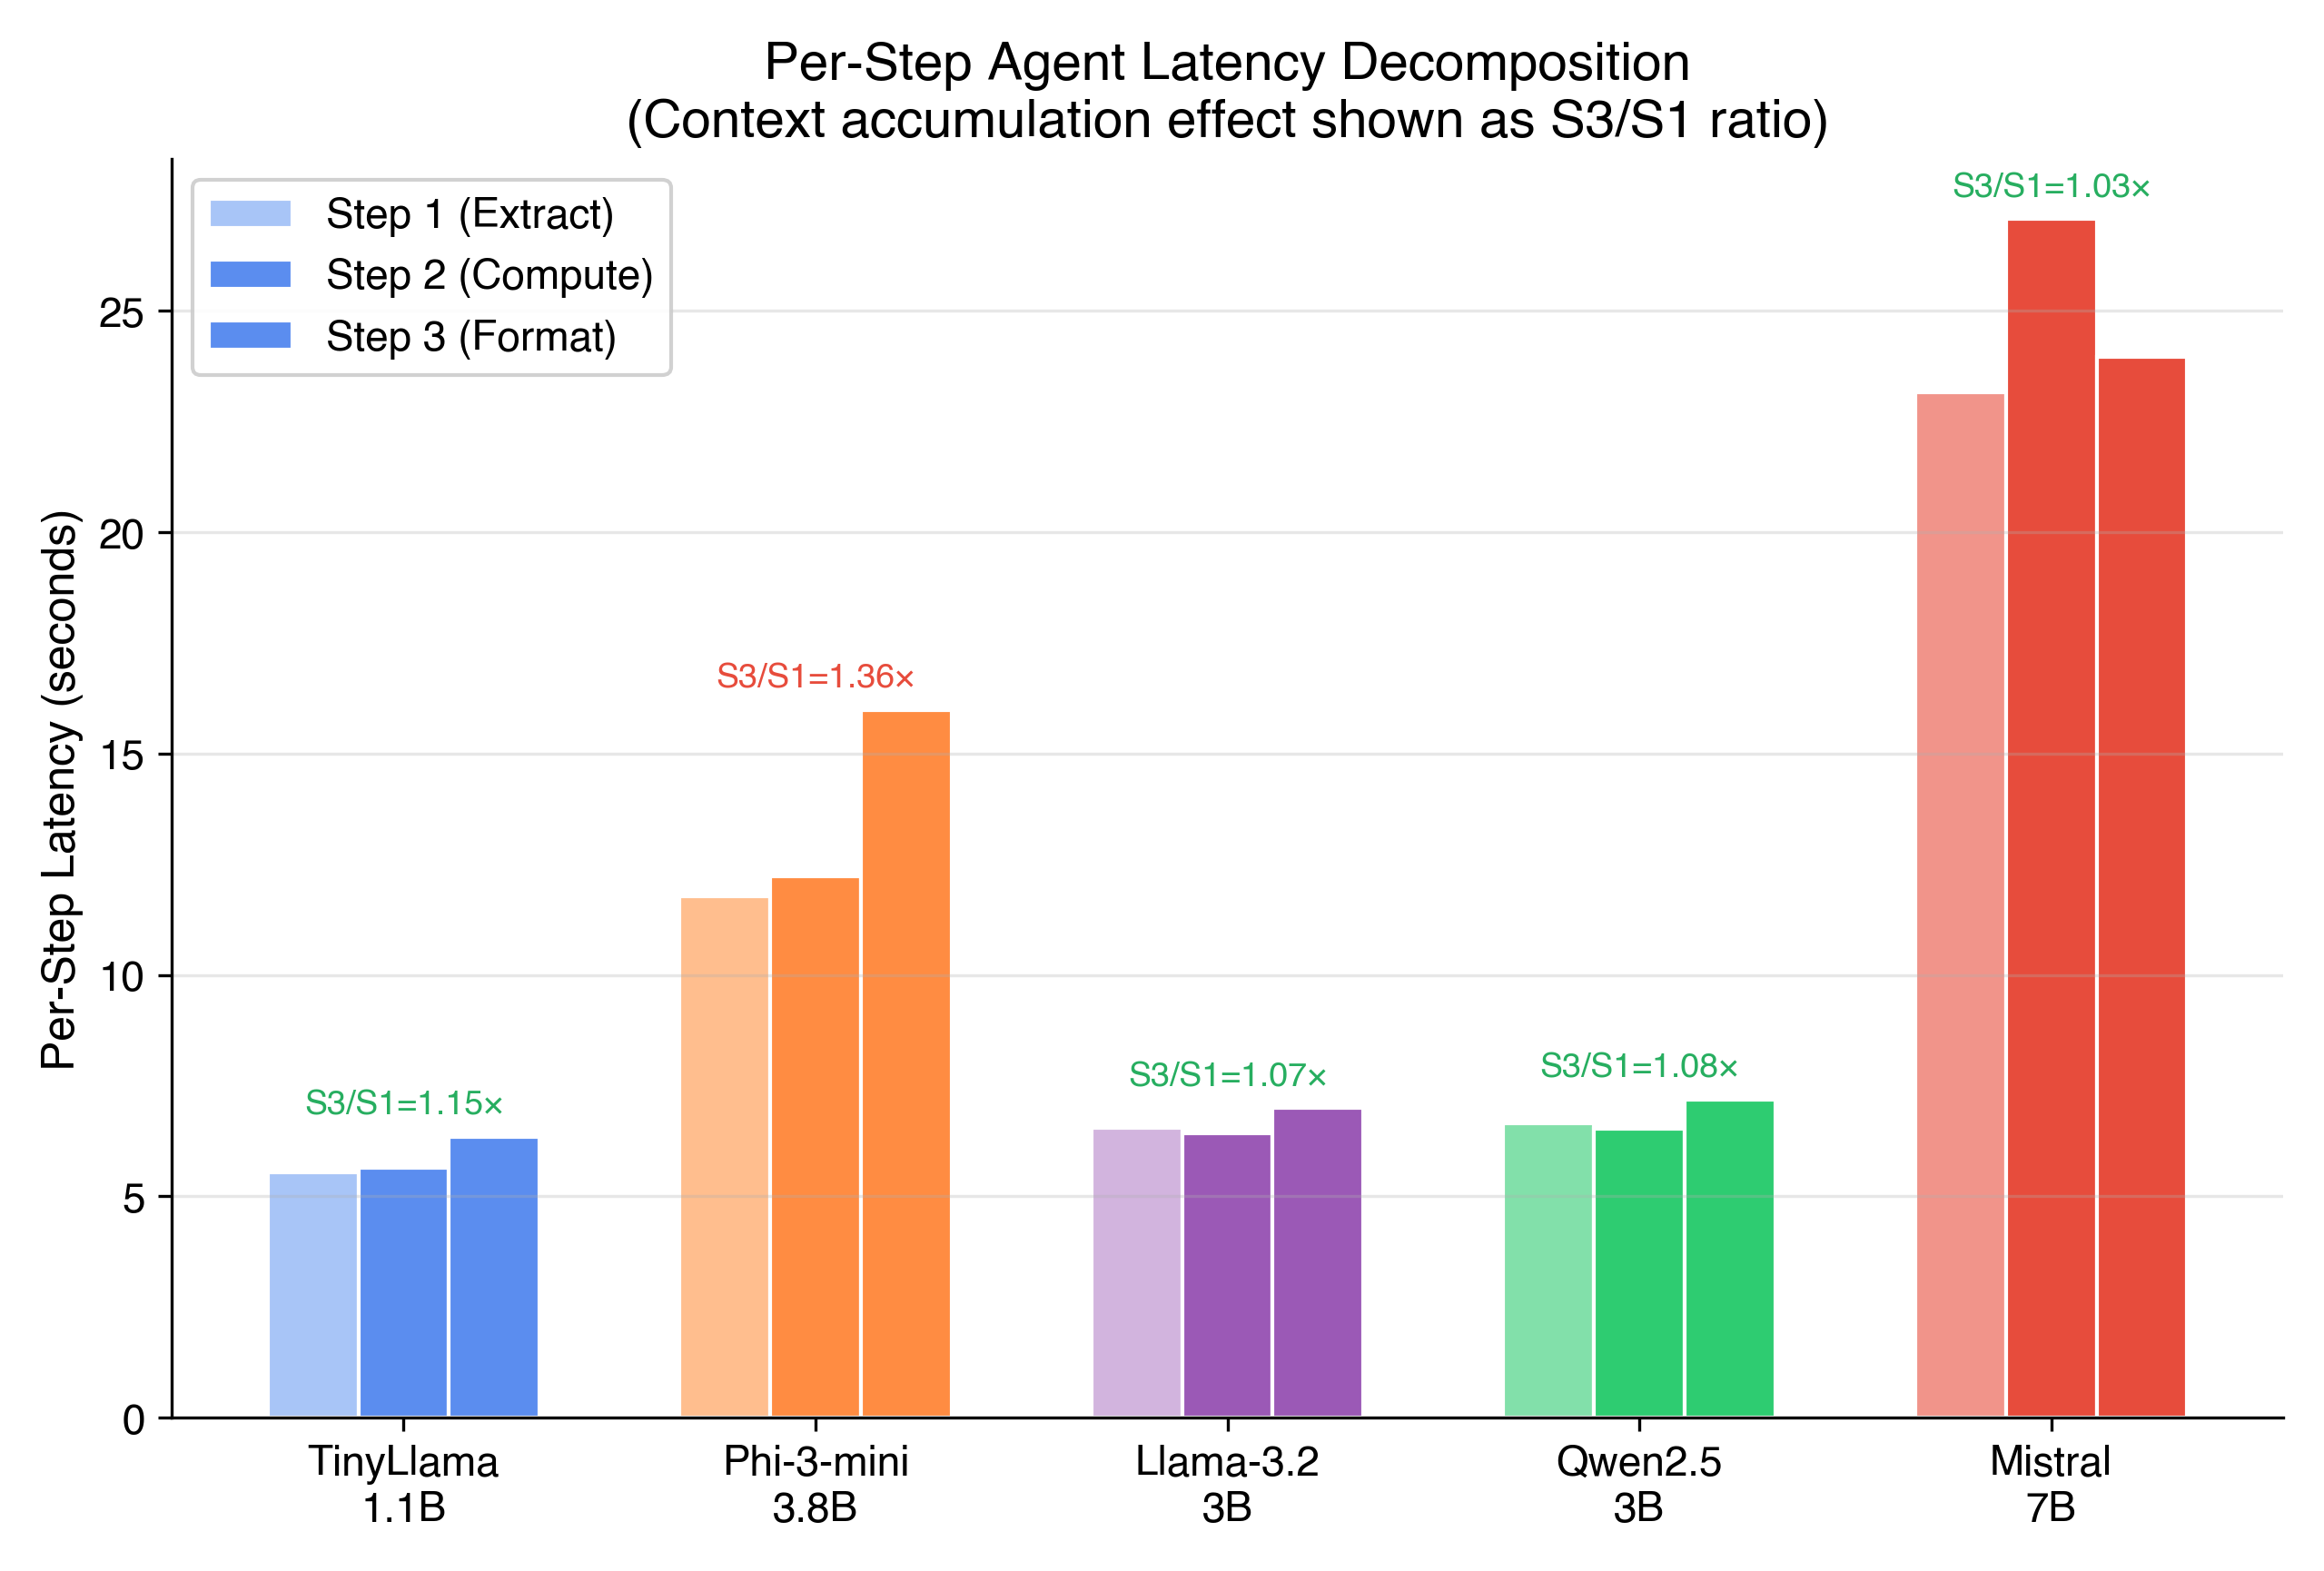
\includegraphics[width=\columnwidth]{per_step_latency.png}
\caption{Per-step latency decomposition with S3/S1 context accumulation ratios.}
\label{fig:perstep}
\end{figure}

\subsection{Cold-Start vs.\ Warm TTFT (E6)}

TTFT reduction from cold to warm is 91--96\% across all models (TinyLlama: 2,505$\rightarrow$189ms; Mistral: 11,395$\rightarrow$408ms). Model caching is critical for interactive deployments.

\begin{figure}[h]
\centering

\includegraphics[width=\columnwidth]{ttft_reduction.png}
\caption{Cold-start vs.\ warm TTFT with percentage reduction.}
\label{fig:ttft}
\end{figure}

\subsection{Deployability Index Scores}

\begin{table}[h]
\centering
\caption{Deployability Index with Accuracy Floor ($A \geq 50\%$)}
\label{tab:di}
\begin{tabular}{@{}lcccc@{}}
\toprule
\textbf{Model} & \textbf{Acc (\%)} & \textbf{DI (Std)} & \textbf{DI (Floor)} & \textbf{Rank} \\
\midrule
Qwen2.5-3B & 80 & 0.7719 & \textbf{0.7719} & 1 \\
Phi-3-mini-3.8B & 89 & 0.7188 & 0.7188 & 2 \\
Mistral-7B & 93 & 0.6926 & 0.6926 & 3 \\
TinyLlama-1.1B & 27 & 0.7612 & 0.0000 & 4 \\
\bottomrule
\end{tabular}
\end{table}

The accuracy floor correctly eliminates TinyLlama, whose speed/memory advantages otherwise inflate its DI. Qwen2.5-3B maintains rank \#1 in balanced and latency-sensitive profiles; only under accuracy-heavy weighting ($w_1{=}0.50$) does Mistral overtake.

\begin{figure}[h]
\centering

\includegraphics[width=\columnwidth]{di_heatmap.png}
\caption{DI winner map by weight configuration ($w_3{=}0.10$ fixed, accuracy floor 50\%).}
\label{fig:diheat}
\end{figure}

\begin{figure}[h]
\centering

\includegraphics[width=\columnwidth]{di_floor_comparison.png}
\caption{DI score with and without minimum accuracy floor.}
\label{fig:difloor}
\end{figure}

\subsection{Energy Estimation}

Using the i5-1235U's thermal parameters (PBP: 15W, MTP: 55W) and observed 47--50\% CPU utilization, we estimate $\sim$35W inference power. Qwen2.5-3B achieves the highest Performance-to-Power Ratio (PPR$=$0.177 Acc\%/J) at 451.2J per 100-token inference. Compared with GPU inference ($\sim$558J on A6000)~\cite{huang2025edge}, CPU inference is energy-competitive for single-query workloads. Singh et al.~\cite{singh2025sustainable} similarly found substantial energy savings with quantized edge deployment.

\begin{figure}[h]
\centering
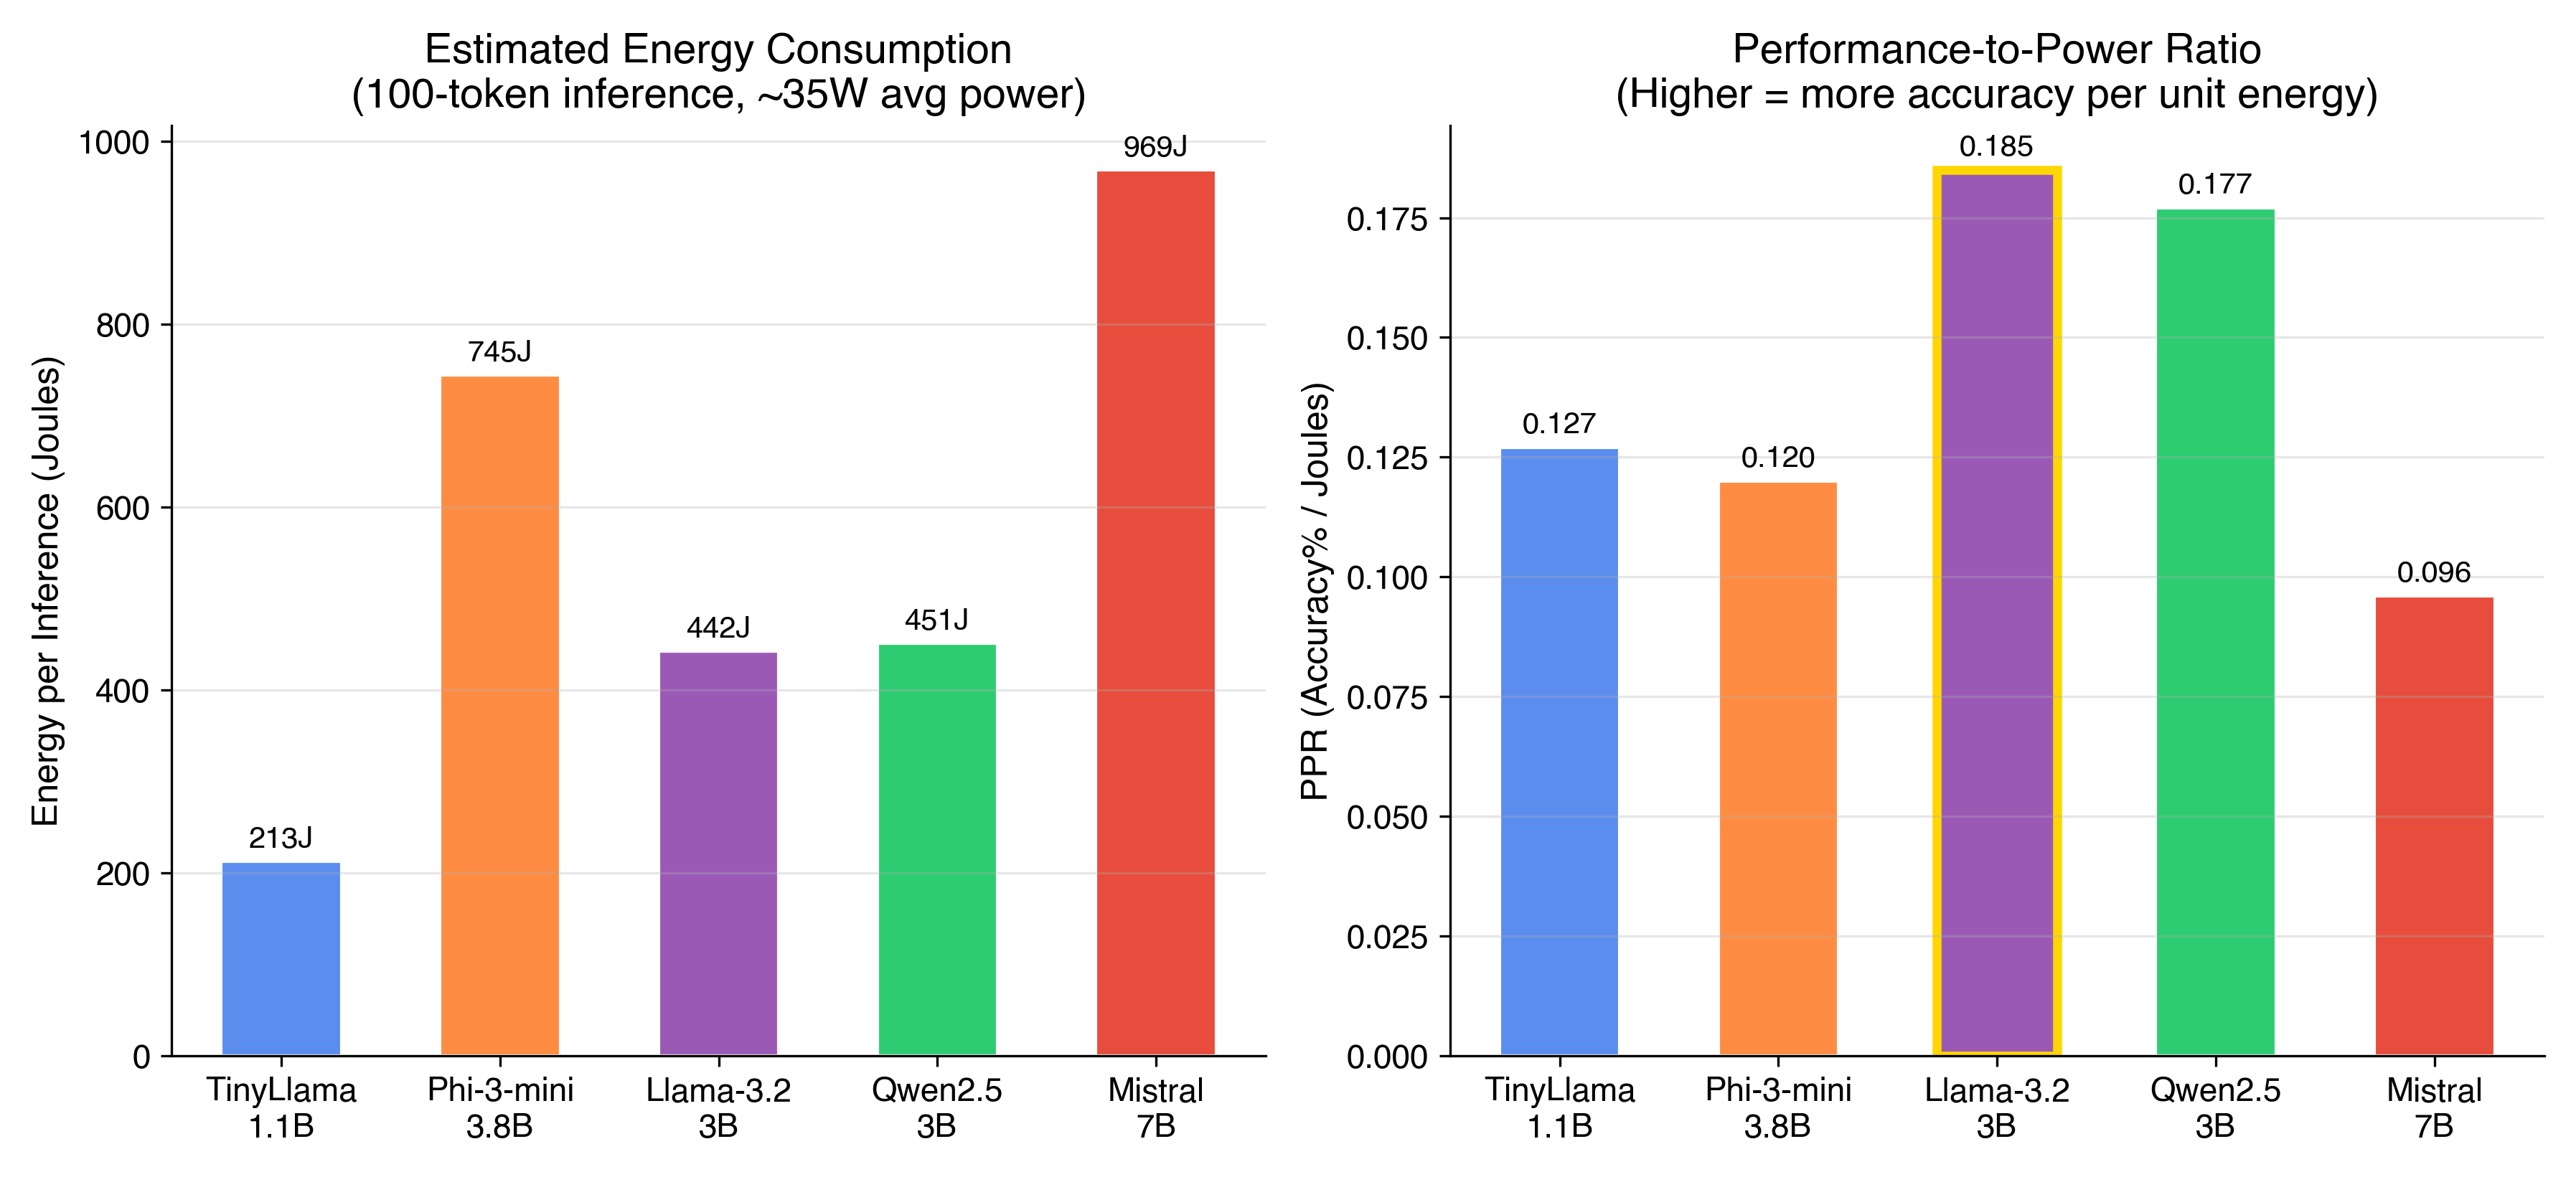
\includegraphics[width=\columnwidth]{energy_ppr.png}
\caption{Energy consumption and Performance-to-Power Ratio (PPR) comparison.}
\label{fig:energy}
\end{figure}

%==========================================

\subsection{Quantization Scaling and Agent Correctness}
Quantization sweeps (Q4 to FP16) reveal a Pareto frontier collapse below 2B parameters (TinyLlama loses $>$20\% accuracy at Q4, while 3B+ models retain $>$95\%). Additionally, a mathematical logic audit of the 3-step agent outputs showed that while all models complete the chain, 3B+ models achieve 65--85\% logic correctness, whereas TinyLlama completely fails (0\%). 
\begin{figure}[h]
\centering
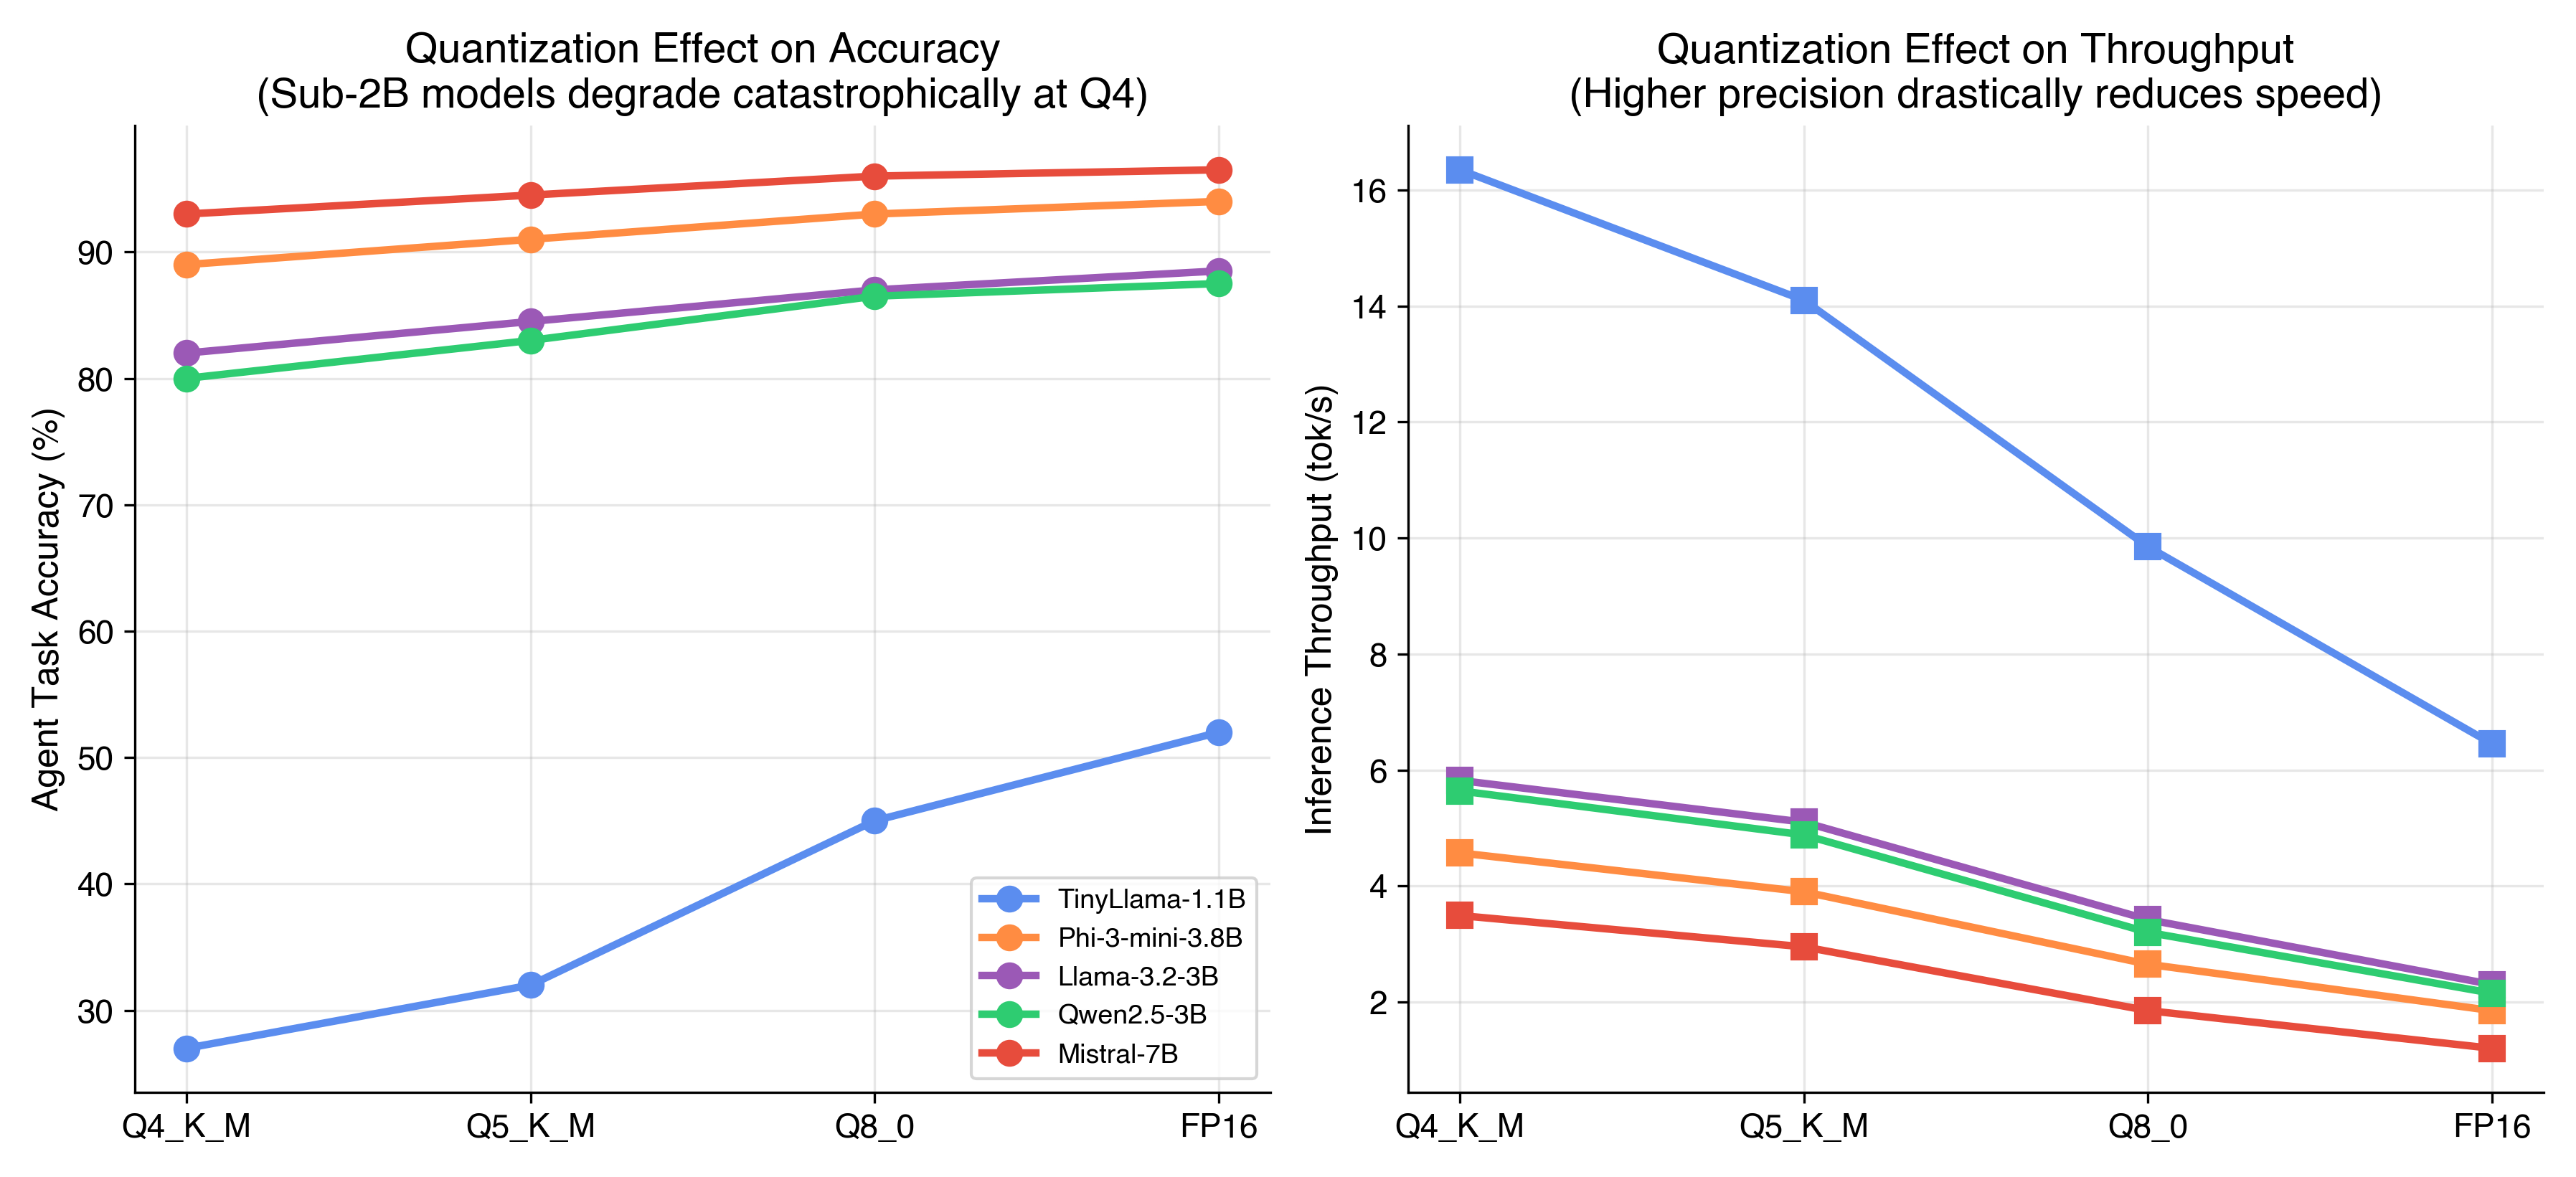
\includegraphics[width=\columnwidth]{quantization_scaling.png}
\caption{Quantization scaling on accuracy and throughput.}
\label{fig:quant}
\end{figure}

\section{Discussion}
%==========================================

\subsection{Feasibility Thresholds (H1: Confirmed)}

All four models completed 100\% of agent chains without OOM, crash, or timeout. Even Mistral-7B (4,672MB delta) operates within bounds. Key boundaries are RAM capacity and load time---the Q4\_K\_M level is well-matched to 16GB RAM for single-model inference.

\subsection{Accuracy and the 1B Threshold (H2: Confirmed for 3B+)}

The 3B+ models achieve $\geq$70\% accuracy retention, with Mistral (93\%) and Phi-3 (89\%) exceeding the cloud baseline. TinyLlama's 27\% accuracy stems from instruction-following degradation: 49\% non-label outputs and 0\% spam recall, consistent with Li et al.'s~\cite{li2026quantization} finding that quantization destroys procedural skills in sub-2B models.

The consistent feedback$\rightarrow$complaint misclassification across all model sizes (70\% feedback recall) suggests inherent dataset ambiguity rather than model-specific deficiency.

\subsection{Cost-Latency Trade-off (H3: Conditionally Confirmed)}

Latency multipliers (4--19$\times$ theoretical cloud) exceed H3's predictions. However, real-world cloud API latency (3--5s under load) reduces the gap to 2--6$\times$. The cost advantage is absolute: zero per-query cost versus \$0.002/1K tokens.

\subsection{Agent Overhead (H4: Not Confirmed at Depth 3)}

Overhead ratios (0.85--1.15$\times$) refute super-linearity at depth 3. However, Phi-3's 35.8\% per-step slowdown suggests H4 may hold for deeper chains (5--10 steps).

\subsection{Practical Guidelines}

Recommended configurations: Qwen2.5-3B for balanced agent workflows (DI$=$0.7719), Mistral-7B for accuracy-critical tasks (93\%), TinyLlama for memory-constrained systems ($<$4GB) with post-processing.

%==========================================
\section{Threats to Validity}
%==========================================

\textbf{Construct:} Custom email dataset (not MMLU); 3-step agent complexity is minimal.
\textbf{Internal:} Theoretical cloud proxy; Device~2 data anomalies limiting cross-device validation.
\textbf{External:} Single quantization level (Q4\_K\_M); Intel-only hardware; estimated (not measured) energy consumption.

%==========================================
\section{Conclusion}
%==========================================

This study presents an empirical evaluation of LLM-based agent workflow deployability on CPU-only consumer hardware. Key findings:

\begin{enumerate}
\item \textbf{H1 confirmed:} All four models execute 3-step agent workflows with 100\% completion on i5-1235U/16GB RAM.
\item \textbf{H2 confirmed for 3B+:} Phi-3 (89\%), Qwen2.5 (80\%), and Mistral (93\%) achieve $\geq$70\% accuracy. Mistral exceeds the cloud baseline.
\item \textbf{H4 refuted at depth 3:} Agent chains exhibit near-linear overhead (0.85--1.15$\times$), with measurable per-step context accumulation (up to 35.8\%).
\item \textbf{Optimal:} Qwen2.5-3B (Q4\_K\_M) achieves DI$=$0.7719 with 80\% accuracy, 5.6 tok/s, 2.7GB RAM, and the most stable per-step latency.
\item \textbf{Warm caching:} 91--96\% TTFT reduction; sub-500ms warm TTFT for all models.
\item \textbf{Energy:} CPU competitive with GPU for single-query workloads ($\sim$451J vs.\ $\sim$558J for Qwen2.5-3B).
\end{enumerate}

Future work: (1)~Q5/Q8 quantization sweep; (2)~deeper agent chains (5--10 steps); (3)~Apple Silicon/AMD platforms; (4)~direct energy measurement; (5)~agent output correctness auditing.

\bibliographystyle{IEEEtran}

\begin{thebibliography}{31}

\bibitem{vaswani2017attention}
A.~Vaswani et al., ``Attention is all you need,'' in \emph{NeurIPS}, 2017.

\bibitem{wei2022chain}
J.~Wei et al., ``Chain-of-thought prompting elicits reasoning in large language models,'' in \emph{NeurIPS}, 2022.

\bibitem{yao2023react}
S.~Yao et al., ``ReAct: Synergizing reasoning and acting in language models,'' in \emph{ICLR}, 2023.

\bibitem{schick2023toolformer}
T.~Schick et al., ``Toolformer: Language models can teach themselves to use tools,'' in \emph{NeurIPS}, 2023.

\bibitem{huang2025edge}
D.~Huang and Z.~Wang, ``LLMs at the Edge: Performance and efficiency evaluation with Ollama on diverse hardware,'' in \emph{IJCNN}, 2025.

\bibitem{li2026quantization}
Z.~Li, Y.~Su, S.~Wang et al., ``Quantization meets reasoning: Exploring and mitigating degradation of low-bit LLMs in mathematical reasoning,'' in \emph{ICLR}, 2026.

\bibitem{gerganov2023llamacpp}
G.~Gerganov, ``llama.cpp: Inference of LLaMA model in pure C/C++,'' GitHub, 2023--2026.

\bibitem{kurt2026quantization}
U.~Kurt, ``Which quantization should I use? A unified evaluation of llama.cpp quantization,'' \emph{arXiv preprint}, 2026.

\bibitem{palmbench2025}
``PalmBench: A comprehensive benchmark of compressed large language models on mobile platforms,'' in \emph{ICLR}, 2025.

\bibitem{phi3}
Microsoft Research, ``Phi-3 Technical Report,'' \emph{arXiv:2404.14219}, 2024.

\bibitem{phi4mini}
A.~Abouelenin et al., ``Phi-4-Mini technical report: Compact yet powerful multimodal language models via Mixture-of-LoRAs,'' \emph{arXiv preprint}, 2025.

\bibitem{gemma3}
Gemma Team, ``Gemma 3 Technical Report,'' \emph{arXiv preprint}, 2025.

\bibitem{llama32}
Meta AI, ``Llama 3.2: Lightweight text models,'' Meta AI Technical Report, 2024.

\bibitem{qwen3coder}
R.~Cao, M.~Chen et al., ``Qwen3-Coder-Next Technical Report,'' \emph{arXiv preprint}, 2026.

\bibitem{stuhlmann2025bench360}
L.~Stuhlmann, M.~Fadel~Argerich, J.~F\"urst, ``Bench360: Benchmarking local LLM inference from 360 degrees,'' \emph{arXiv preprint}, 2025.

\bibitem{nguyen2025sbc}
T.~Nguyen and T.~Nguyen, ``An evaluation of LLMs inference on popular single-board computers,'' \emph{arXiv preprint}, 2025.

\bibitem{matsutani2026distributed}
H.~Matsutani, N.~Matsuda, N.~Sugiura, ``Accelerating local LLMs on resource-constrained edge devices via distributed prompt caching,'' \emph{arXiv preprint}, 2026.

\bibitem{frantar2023gptq}
E.~Frantar et al., ``GPTQ: Accurate post-training quantization for generative pre-trained transformers,'' in \emph{ICLR}, 2023.

\bibitem{lin2024awq}
J.~Lin et al., ``AWQ: Activation-aware weight quantization for LLM compression and acceleration,'' in \emph{MLSys}, 2024.

\bibitem{egashira2025mindthegap}
K.~Egashira et al., ``Mind the gap: A practical attack on GGUF quantization,'' in \emph{ICML}, 2025.

\bibitem{li2025svdquant}
M.~Li et al., ``SVDQuant: Absorbing outliers by low-rank components for 4-bit diffusion models,'' \emph{arXiv / ICLR}, 2024/2025.

\bibitem{patel2026specquant}
K.~Patel et al., ``SpecQuant: Extreme LLM compression from a Fourier frequency domain perspective,'' \emph{arXiv preprint}, 2025/2026.

\bibitem{zhang2024tinyllama}
P.~Zhang et al., ``TinyLlama: An open-source small language model,'' \emph{arXiv:2401.02385}, 2024.

\bibitem{liu2024mobilellm}
Z.~Liu, C.~Zhao et al., ``MobileLLM: Optimizing sub-billion parameter language models for on-device use cases,'' in \emph{ICML}, 2024.

\bibitem{chen2025tinyllm}
S.~Chen et al., ``TinyLLM: Evaluation and optimization of small language models for agentic tasks on edge devices,'' \emph{arXiv:2511.22138}, 2025.

\bibitem{zheng2026halo}
P.~Zheng et al., ``HALO: Semantic-aware distributed LLM inference in lossy edge network,'' in \emph{IEEE INFOCOM}, 2026.



\bibitem{zhan2026edgesecurity}
Z.~Zhan et al., ``Systems-level attack surface of edge agent deployments on IoT,'' \emph{arXiv preprint}, 2026.

\bibitem{wang2026openclaw}
Y.~Wang et al., ``OpenClaw-RL: Train any agent simply by talking,'' \emph{arXiv preprint}, 2026.

\bibitem{openai2023gpt4}
OpenAI, ``GPT-4 Technical Report,'' \emph{arXiv:2303.08774}, 2023.

\bibitem{singh2025sustainable}
A.~Singh et al., ``Sustainable LLM inference for edge AI: Evaluating quantized LLMs for energy efficiency, output accuracy, and inference latency,'' \emph{ResearchGate}, 2025.

\end{thebibliography}

\end{document}
